\todo{ Some words about the genetics accelerator + Image of architecture of Genetic Pipeline?}
The galapagos architecture includes a highly specialised pipeline for performing genetic operations. The pipeline is based on the observation that selection, crossover, and mutation works similar for a specific subset of problems. These can therefore be implemented as hardware accelerators constructed for performing one specific task. Constructing such accelerators has been proven to be very beneficial regarding performance. \todo{ Should somehow be documented?} Designing specialised hardware is usually simpler and thereby more effective than constructing general purpose components. This pipeline will effectively relieve the general cores, the fitness cores, from performing the evolution of individuals. The idea is that these will make the fitness cores able to only focus on the computation of fitness ranking, which is considered computational intensive. In the mean time the \emph{genetic pipeline} can produce new data for ranking. These operations could have been performed by the processor, however, the processor is badly suited for these kind of operations. Note that the instructions in the pipeline actually uses 5 cycles in order to completely propagate through the pipeline }. It is far better to only use one cycle in order to complete the one specific operation.  

The genetic pipeline is constructed with three types of specialised cores for performing selection, crossover, and mutation. These are operations that occurs frequently in genetic algorithms. These are connected to two internal memory banks on the \emph{FPGA}, namely the unrated and rated pool.

In the selection core, on the other hand, the core needs to be able to access the data bus very frequently in order maximize the throughput.
Since fitness calculation can be assumed to be computationally bound, the data bus is more or less available for the selection core.
This allows the genetic pipeline to compute the chromosomes required for the next step before they are required by the fitness cores. 


-Abstraction for the programmer. Simpler to program.
-Do not need components like ALU
- effective 
- Less control over the genetic pipeline
- \todo{ Does the original writer feel that these points are well enough covered, so that I or someone may remove them? :) }

\begin{figure}

  \centering
  % Trim er [left bottom right top]
  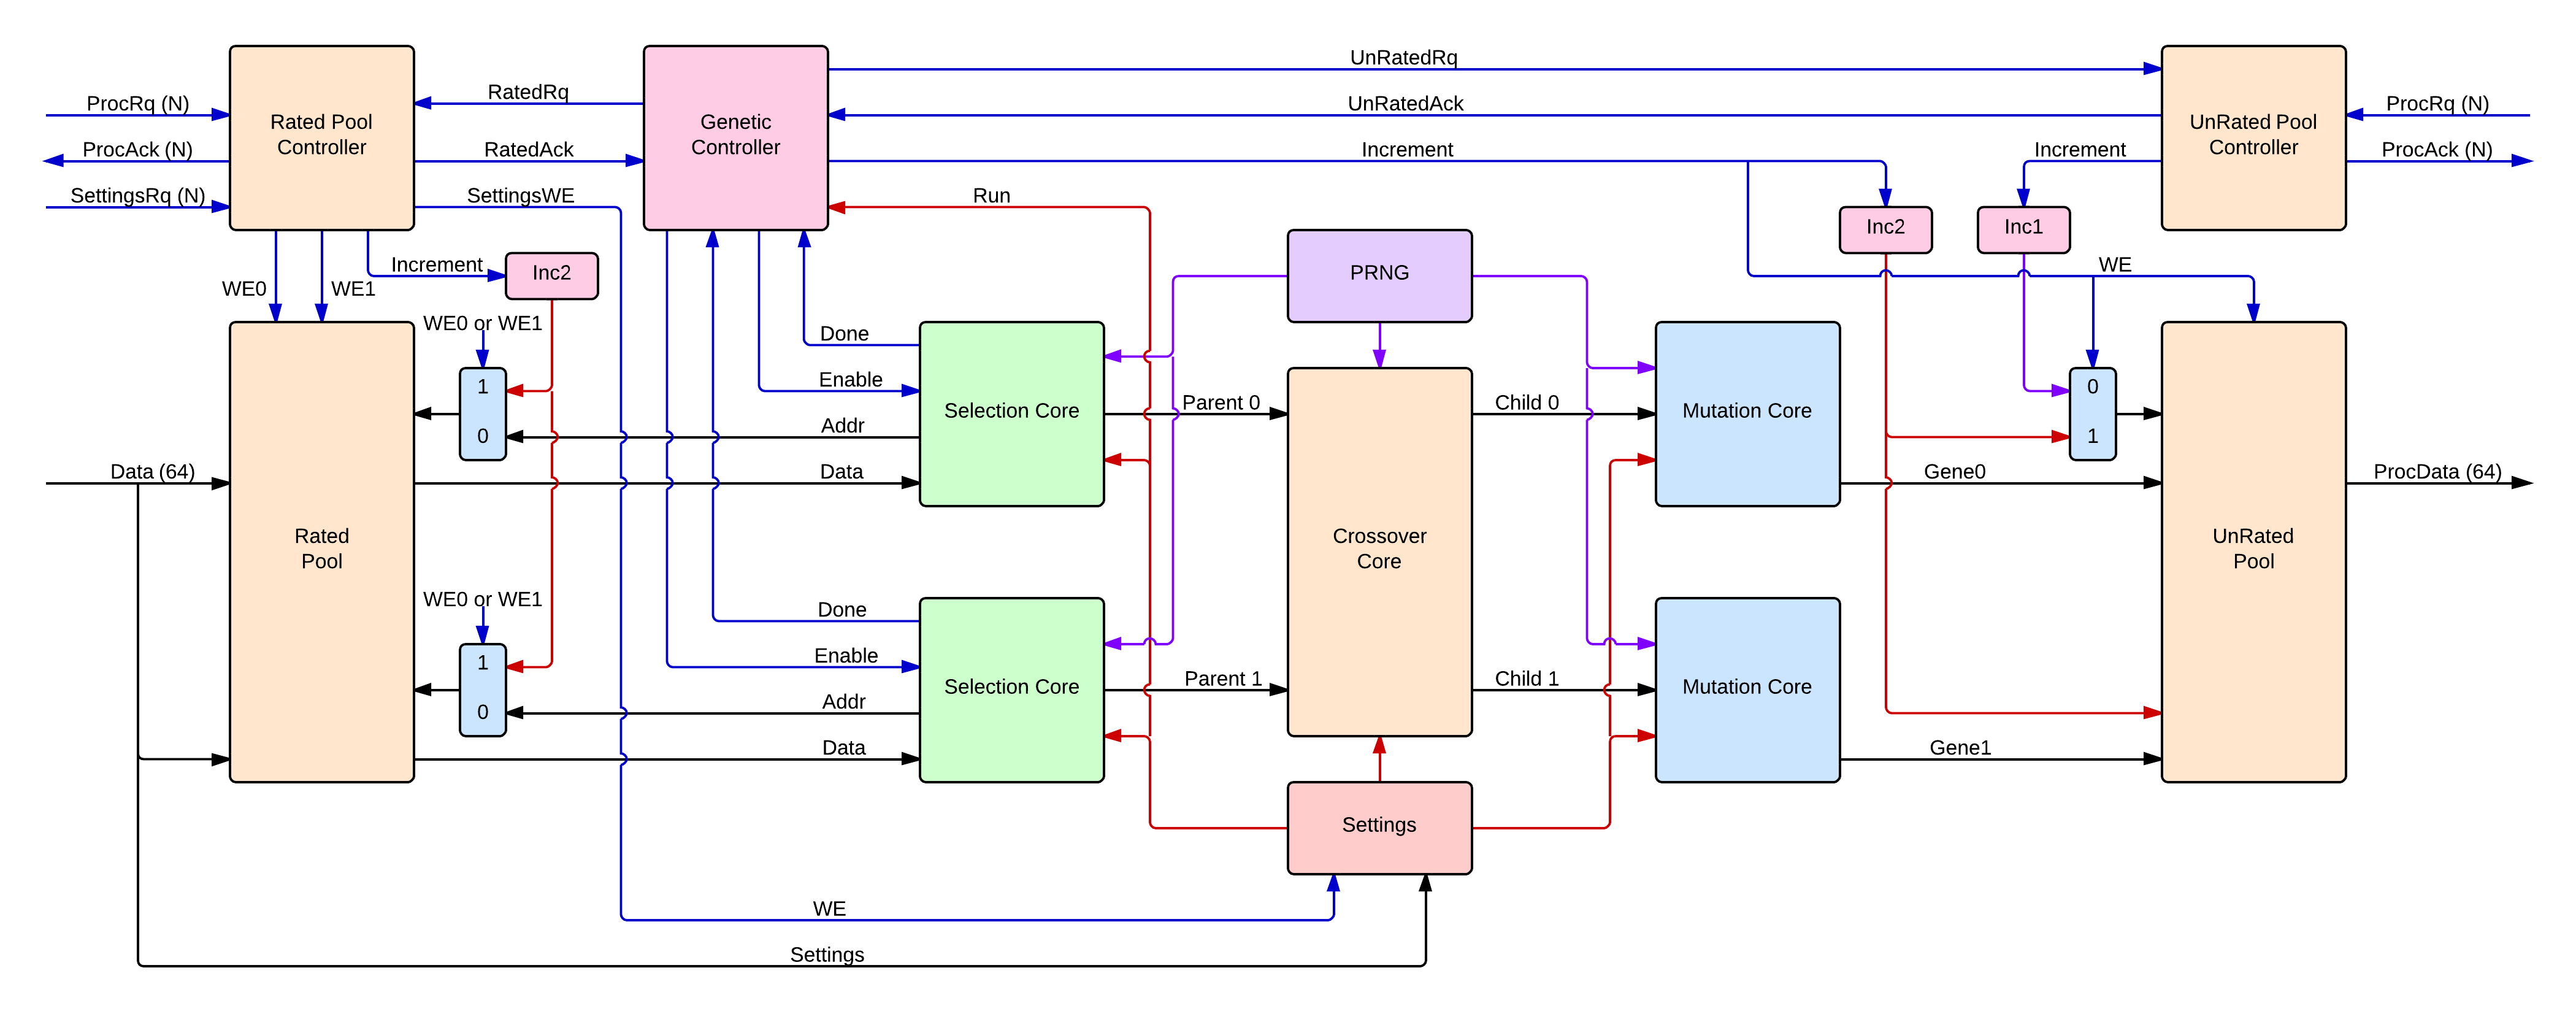
\includegraphics[width=\textwidth]{fpga/fig/genetic_pipeline.png}
  \caption{Genetic pipeline architecture}
  \label{fpga:fig:genetic:genetic_pipeline}
\end{figure}




\todo{Should include architecture graphic of the Genetic Pipeline}

\subsubsection {Selection Core} \label{fpga:selection:ss:selection_core}
    \subsection {Design of the selection core} \label{fpga:selection:ss:selection_core}

The selection core is designed based on a tournament selection algorithm. It is designed to select an chromosome from a random position in the rated pool. The current best and the random selected is compared to each other with use of an comparator. The best chromosome is stored and used in the next tournament round. After some number of tournaments the current best is transferred to the crossover core. The selection core is actually responsible for letting the rest of the genetic pipeline know when it can fetch the next chromosome. 

The selection core is designed with efficiency in mind. The overall time spent in the genetic pipeline must be smaller than the time spent ranking the chromosomes. Note that the fitness cores are connected to the same memory bus as the genetic pipeline. This could potentially lead to a memory bottleneck resulting in starvation. The selection core tries to overcome this fact by reducing the memory access to a minimum. Note that the selection core has reserved the memory bus during the ongoing tournament. This implies that port used by the selection core is unavailable to others during this time. It is designed to not use the memory more than it absolutely have to. For instance, if the current fitness value is greater than the fitness value just fetched. The selection core will not bother fetching the accompanying chromosome. Ensuring that the memory resources are not wasted. This is accomplished with an \emph{state machine}. 



\subsubsection{Data Path}
Upon the beginning of the data path design, the group wanted to determine the the components required to perform the selection. In this specific case the group decided to design a data path able to perform a tournament selection. The resulting architecture is made as simple as possible.  It is composed of \emph{flip flops}, \emph{control unit} and an \emph{comparator}. The different components are connected as seen in figure.




\fxnote{Add figure of selection core}


\subsubsection{Control Unit} \label{fpga:selection:sss:control_unit}



\subsubsection {Comparator} \label{fpga:selection:sss:comparator}



\subsubsection{Case study} \label{fpga:selection:sss:case_study}



 \label{fpga:subsection:selection_core}

\subsubsection{Crossover Core} \label{fpga:crossover:ss:crossover_core}
    The crossover Core is the next part in the genetics accelerator after the selection cores. Two inputs are forwarded from the two selections cores as "parents", and two outputs are the "children" of the inputs, containing bits from both parents. All the bits from both the parents are forwarded in the children, but in some parts the bit-patterns are switched on the children, based a selected crossover function and on a random input from the PRNG. Henceforth this is called crossover.

There are three distinct crossover functions that are implented: Split, doublesplit and function.

\paragraph{\textit{Split Fucntion}}
\begin{figure}[H]
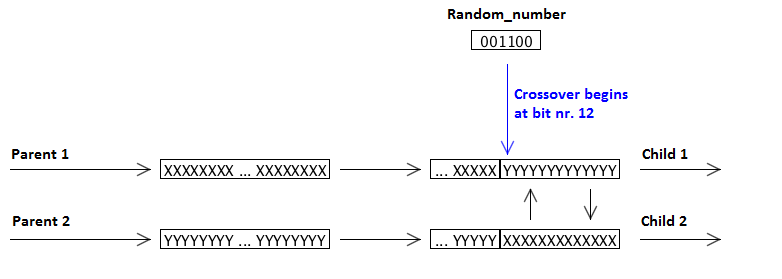
\includegraphics[width=\textwidth]{fpga/fig/crossover_split.png}
\caption{Crossover split function}
\label{fig_crossover_split}
\end{figure}

The first function, crossover split, performs crossover from a selected bit number in the children and until the edge (bit number 0). This can be seen in figure \ref{fig_crossover_split}. The values in the parents are represented with X's and Y's, and a single X or Y can have the value 0 or 1, independent of each other.
The bit number for starting crossover is based on the value of a 6-bit input random\_number, which is provided by the PRNG. This value ranges from 0 to 63.

\todo Describe how it technically works??

\paragraph{\textit{Double-split Fucntion}}
\begin{figure}[H]
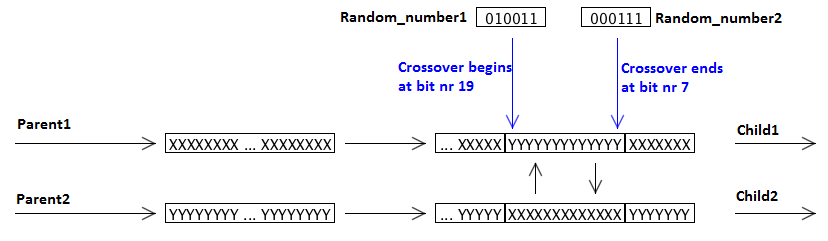
\includegraphics[width=\textwidth]{fpga/fig/crossover_doublesplit.png}
\caption{Crossover double-split function}
\label{fig_crossover_doublesplit}
\end{figure}

The second function, crossover double-split, is similar to the crossover\_split-function, but in additionally to having a starting bit for crossover, it also has an ending bit where the crossover starts, instead of reaching the edge at bit nr. 0. PRNG provides with 2 6-bit inputs, random\_number1 and random\_number2, whose values selects the starting bit and the ending bit for the crossover. These values range from 0 to 63, and if both are the same, then only one bit will be selected for crossover.

\todo Describe how it technically works??

\paragraph{\textit{XOR Fucntion}}
\begin{figure}[H]
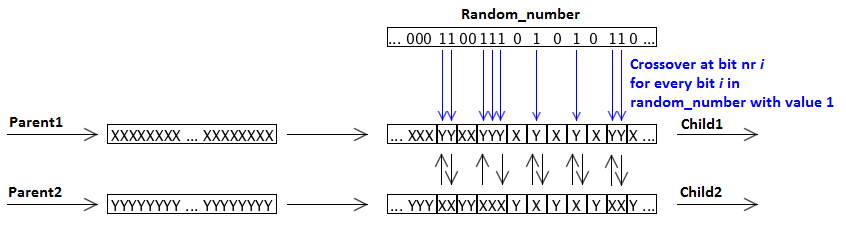
\includegraphics[width=\textwidth]{fpga/fig/crossover_xor.png}
\caption{Crossover XOR function}
\label{fig_crossover_xor}
\end{figure}

The third function, crossover XOR, performs crossover bit by bit, based on the 64-bit input random\_number. For each bit number \textit{i} in random\_number that has the value 1, the function will perform crossover on the children at the same bit number \textit{i}. This function is called XOR because of use of XOR-gates in earlier version of the function, and the principle is still the same: For each bit number \textit{i} in the child, the value will the bit number \textit{i} from one and only one parent. And which parent it is depends on the value of bit number \textit{i} in random\_number.

\todo Describe how it technically works??

\paragraph{\textit{Crossover Core Toplevel}}

The crossover core is implemented on the genetics accelerator as a toplevel containing 3 subcores, one for each function, as well as a fourth path with no crossover. In addition to the two parent inputs and 64-bit input random\_number, the toplevel has a control\_number input used for determining which crossover function is to be used: Split, doublesplit, xor, "party mode" or no crossover at all. Party mode is choosing crossover function at random, based on the 2 LS bits in the random\_number. In this way, whenever inputs are sent through the crossover\_toplevel, different functions may be used at different times. These are the control values:
\begin{itemize}
\item 000 - Split
\item 001 - Double-split
\item 010 - XOR
\item 011 - No crossover
\item 1XX - Party mode, in which case these are the random control values:
    \begin{itemize}
    \item 00 - Split
    \item 01 - Doublesplit
    \item 10 - XOR
    \item 11 - No crossover
    \end{itemize}
\end{itemize} \label{fpga:subsection:crossover_core}

\subsubsection{Mutation Core}\label{fpga:mutation:ss:mutation_core}
    The mutation core is the final part in the genetics accelerator. The mutation core takes in a forwarded child from the crossover core as input and may perform mutation on a few selected bits before passing on the result. 

\begin{figure}[H]
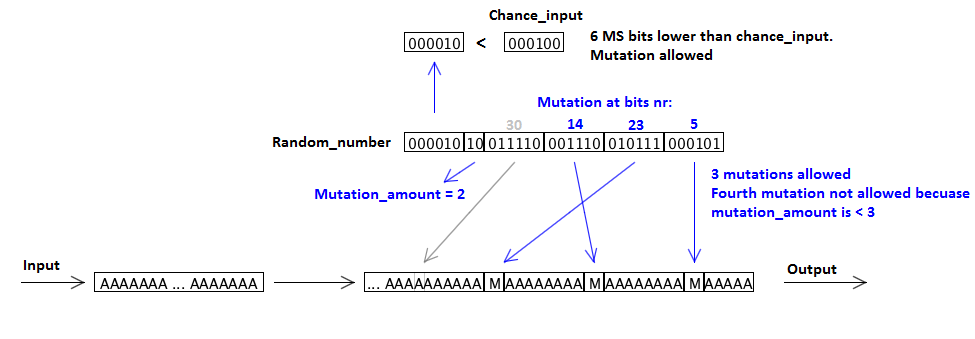
\includegraphics[width=\textwidth]{fpga/fig/mutation.png}
\caption{Mutation core function concept}
\label{Fig_Mutation}
\end{figure}

In addition to the the 64-bit child, the mutation core also takes in a 32-bit random\_number and a 6-bit chance\_input as inputs. As it can be seen in the example in figure \ref{Fig_Mutation}, all bits that are not mutated are represented by an A, and mutated bits are represented with M. The values in each A or M can be 0 or 1, independent of each other. The value M at bit number \emph{i} is the opposite of the original value A at same bit number \emph{i} in the input.
The 6 first bits in the random\_number is compared to the chance\_input, and mutation happens only if the value of these bits are less than the chance input. For each different value in chance\_input, the user may increase or decrease the chance of mutation by about 1,5\%, or $(1 / 2^6)$. If the chance input is set to 000000, no mutation will ever happen, and the user may in this way disable the mutation core.

The next two bits in the random number (bits 25-24) are used to determine how many mutations will happen. There are 4 different values, therefore there can be 1-4 mutations.
The next 24 bits are used to determine which bits are to be mutated. 6 bits are used for finding each bit number. This is similar to what is done in the split and doublesplit functions in the crossover core. These values are numbered, representing their bit field:
\begin{itemize}
\item Nr. 1: 5-0
\item Nr. 2: 11-6
\item Nr. 3: 17-12
\item Nr. 4: 23-18
\end{itemize}
These are numbered after the amount of allowed mutation. Nr. 1 will always happen when a mutation occurs, while nr. 4 happens only when the amount\_number allows for 4 mutations.

Note that if more than one of these numbers point to the same bit to be mutated, the output M will still be the inverted from the original input. For instance, if both numbers 1 and 2 (bits 11-6 and 5-0) have the value 000110, and therefore point at bit number 6, the same mutation will still happen as if only one of these numbers were 000110. If the input bit was 1, the mutated will be 0, and vice versa.
In the example provided in figure \ref{Fig_Mutation}, the 6 first bits of the random\_number are less than the chance\_input, therefore a mutation happens. Bits 23-0 have the values 30, 14, 23 and 5. Because the value of bits 25-24 is 10 (mutation\_amount has value 2), there will be 3 mutations, and the fourth does not occur (though the figure shows where it would have occured if allowed).

\begin{figure}[H]
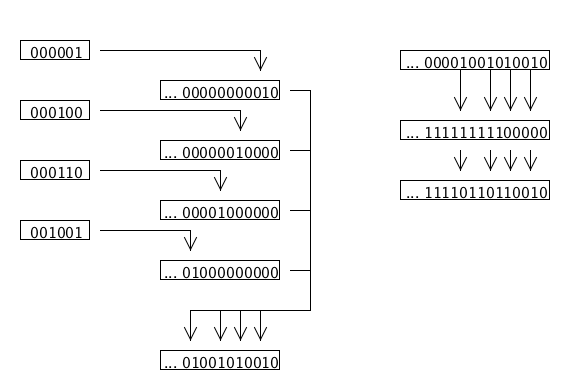
\includegraphics[width=\textwidth]{fpga/fig/mutation_mask.png}
\caption{Setting mutation}
\label{fig_mutation_mask}
\end{figure}

The mutation core is implemented by use of four shifter variables, one for each possible mutation, and set so that only one bit is 1 for the output. A final mutation is set by combining the outputs from the shifter variables by using OR-funftion, and the mutation\_amount determines how many of these outputs are combined. Figure \ref{fig_mutation_mask} shows an example where bits 1, 4, 6 and 9 are set for mutation. In this case the final output is set by combining the input and mutation with the XOR-fuction, so that for each bit \emph{i}, the bit is set to 1 if and only if bit \emph{i} is set in either the input or the mutation, but not both. This can be seen in figure \ref{fig_mutation_perform}.

\begin{figure}[H]
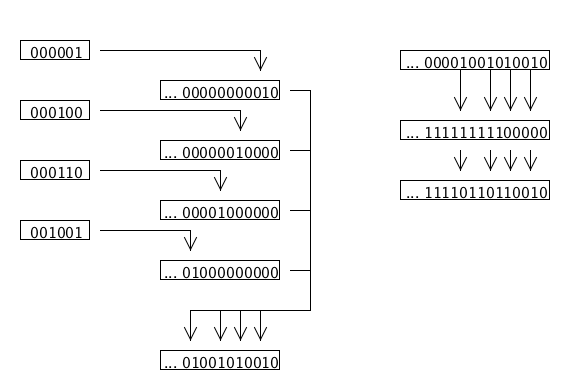
\includegraphics[width=\textwidth]{fpga/fig/mutation_mask.png}
\caption{Performing mutation}
\label{fig_mutation_perform}
\end{figure}

\todo{ "Selected bit number" needs to somehow be defined in the description of the shifter variable + ShifterVariable needs to be described.} \label{fpga:subsection:mutation_core}


